\chapter{Experimentos e Resultados}

Neste Capítulo encontram-se os experimentos realizados com os sistemas devidamente implementados e configurados. Discutiremos os resultados obtidos, testando os sistemas com todas as suas funcionalidades.

\section{Manipulação de usuários}

O microsserviço de usuários utiliza a porta 3001. Para utiliza-lo e testá-lo, devemos utilizar esta porta juntamente com os \textit{endpoints} disponíveis (Seção \ref{sec:usuarios}). Aqui realizaremos as consultas em todos estes \textit{endpoints} e discutiremos os resultados obtidos.

Para criar um usuário devemos consumir\footnote{O termo "consumir um \textit{endpoint}"\  significa enviar informações para o \textit{endpoint}, esperando algum retorno, de sucesso ou falha.} o \textit{endpoint} http://localhost:3001/usuario/cadastrar passando os parâmetros via \textit{POST} no formato \textit{JSON}\footnote{Javascript Object Notation (JSON), é um formato compacto de troca de dados simples e rápida entre sistema}, como na Figura \ref{fig:cadastro}.

A resposta deste \textit{endpoint} pode ser conferida na Figura \ref{fig:cadastro} e, para garantir que o usuário foi incluído no banco de dados, podemos observar a Figura \ref{fig:cadastro}.

\begin{figure}[htbp]
	\centering
	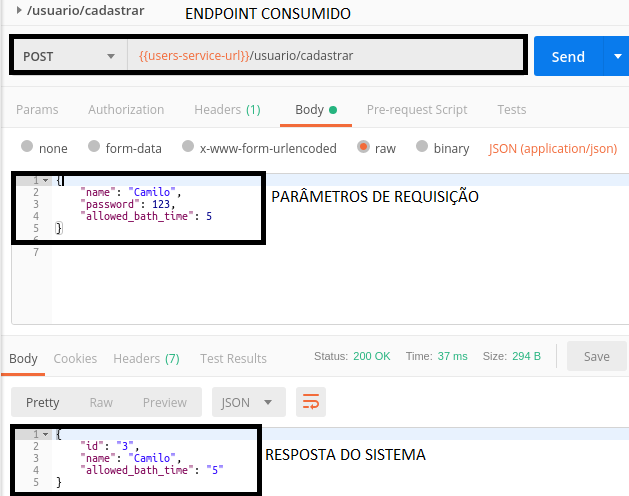
\includegraphics[width=0.7\linewidth]{figuras/postman/cadastro.png}
	\caption{Cadastro de usuários.}
	\label{fig:cadastro}
\end{figure}

\clearpage

O \textit{endpoint} http://localhost:3001/usuario/editar-tempo deve ser consumido para editar o tempo máximo de banho de um usuário (Figura \ref{fig:tempo}). Para editar a senha do usuário, deve-se consumir o \textit{endpoint} http://localhost:3001/usuario/editar-senha (Figura \ref{fig:senha}).

\begin{figure}[htbp]
	\centering
	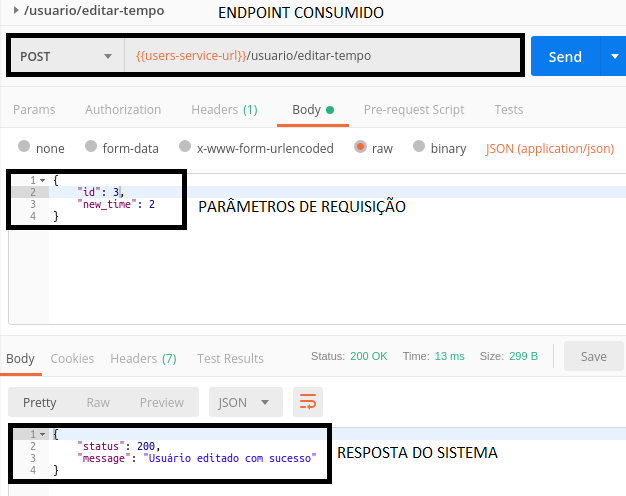
\includegraphics[width=0.7\linewidth]{figuras/postman/time.png}
	\caption{Edição de tempo permitido do usuário.}
	\label{fig:tempo}
\end{figure}

\begin{figure}[htbp]
	\centering
	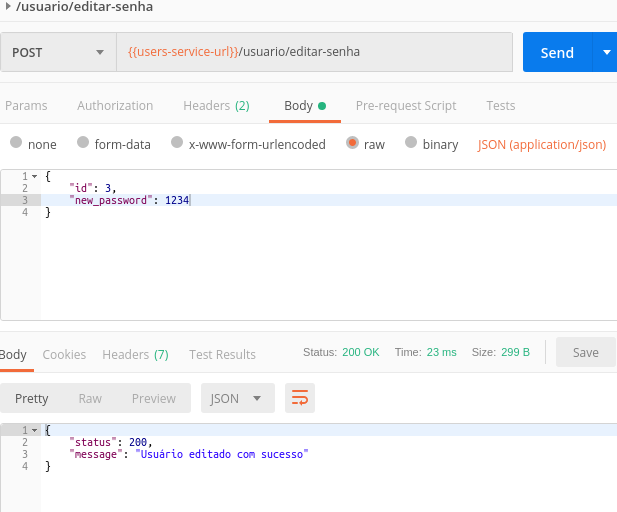
\includegraphics[width=0.7\linewidth]{figuras/postman/password.png}
	\caption{Edição de senha do usuário.}
	\label{fig:senha}
\end{figure}

Conseguimos cadastrar um banho ao consumir o \textit{endpoint} http://localhost:3001/banho via \textit{POST} com os parâmetros e resposta mostrados na Figura \ref{fig:banho}.

\begin{figure}[htbp]
	\centering
	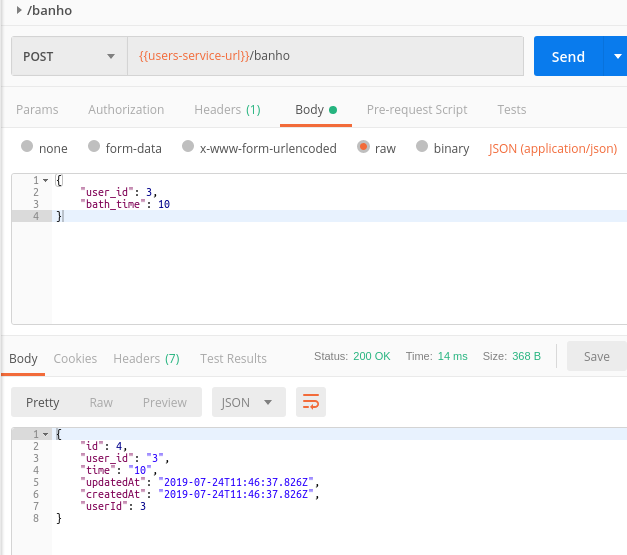
\includegraphics[width=0.7\linewidth]{figuras/postman/bathsinclude.png}
	\caption{Adicionando banhos ao usuário.}
	\label{fig:banho}
\end{figure}

Para recuperar as informações de um usuário, basta consumir o \textit{endpoint} \break http://localhost:3001/usuario/idDoUsuario, com o método \textit{GET}, obtendo o resultado da Figura \ref{fig:usuario}.

\begin{figure}[htbp]
	\centering
	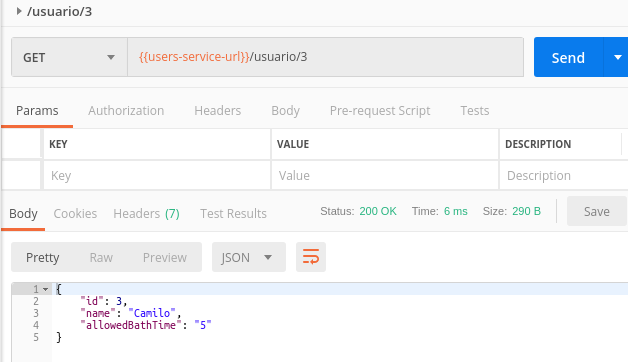
\includegraphics[width=0.7\linewidth]{figuras/postman/getuser.png}
	\caption{Recuperar dados do usuário.}
	\label{fig:usuario}
\end{figure}

Conseguimos as informações de todos os banhos dos usuários consumindo o \textit{endpoint} http://localhost:3001/banho/idDoUsuario, via \textit{GET}, e conseguiremos o resultado exibido na Figura \ref{fig:banhos}.

\begin{figure}[htbp]
	\centering
	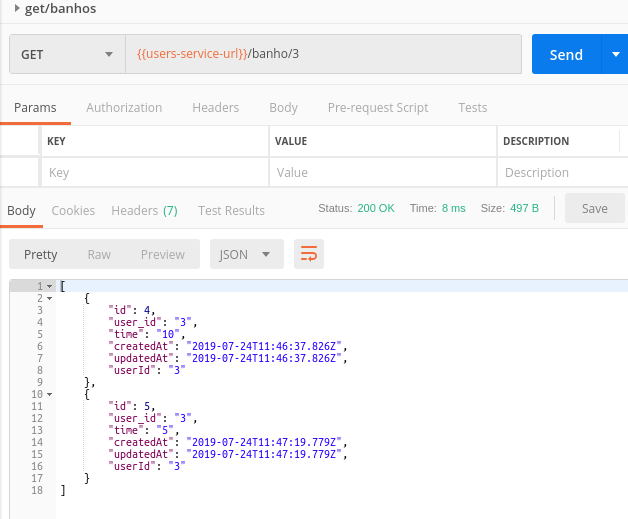
\includegraphics[width=0.7\linewidth]{figuras/postman/getbanhos.png}
	\caption{Recuperar dados de banhos do usuário.}
	\label{fig:banhos}
\end{figure}

Finalmente, podemos autenticar os usuários enviando via \textit{POST} os parâmetros para o \textit{endpoint} http://localhost:3001/usuario/autorizar, obtendo como resposta a Figura \ref{fig:allowedtrue}, para usuário autenticado, e Figura \ref{fig:allowedfalse}, para usuário não autenticado, caso a senha esteja errada.

\begin{figure}[htbp]
	\centering
	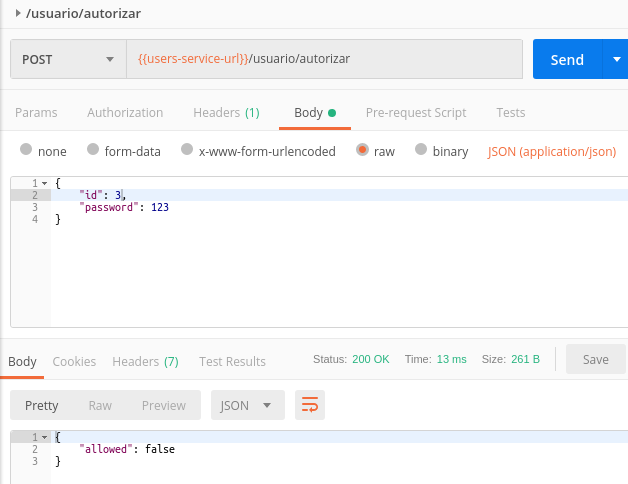
\includegraphics[width=0.7\linewidth]{figuras/postman/allowedfalse.png}
	\caption{Exemplo de usuário não autorizado.}
	\label{fig:allowedfalse}
\end{figure}

\begin{figure}[htbp]
	\centering
	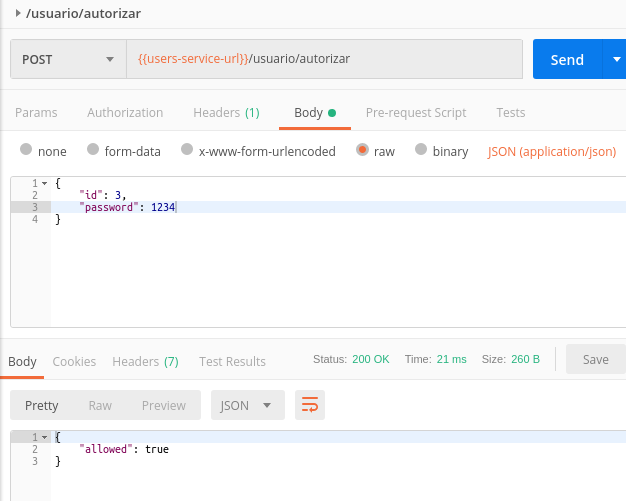
\includegraphics[width=0.7\linewidth]{figuras/postman/allowedtrue.png}
	\caption{Exemplo de usuário autorizado.}
	\label{fig:allowedtrue}
\end{figure}

\section{Visualização via Grafana}

Os dados para a visualização no Grafana foram gerados pelo Sistema de simulação de dados (Seção \ref{sec:sistemasimulacao}).

Ao autenticar um usuário, um sinal é enviado ao tópico do atuador (Seção \ref{sec:valvula}) e o sinal emulado do sensor YF-S201 (Seção \ref{sec:sensor}) inicia a simulação do fluxo, que é automaticamente enviado para o InfluxDB via Sistema de comunicação MQTT (Seção \ref{sec:sistemacomunicacao}), podendo ser visualizado no Grafana. Os gráficos do grafana podem ser acessados via http://localhost:3003, como na Figura \ref{fig:grafanahome}.

Pode ser observado na Figura \ref{fig:grafana-graph} um gráfico do fluxo simulado pelo sensor no horário de 16h40m até 17h00m. Existem dois gráficos com cores diferentes, cada cor é referente a um usuário.

\begin{figure}[htbp]
	\centering
	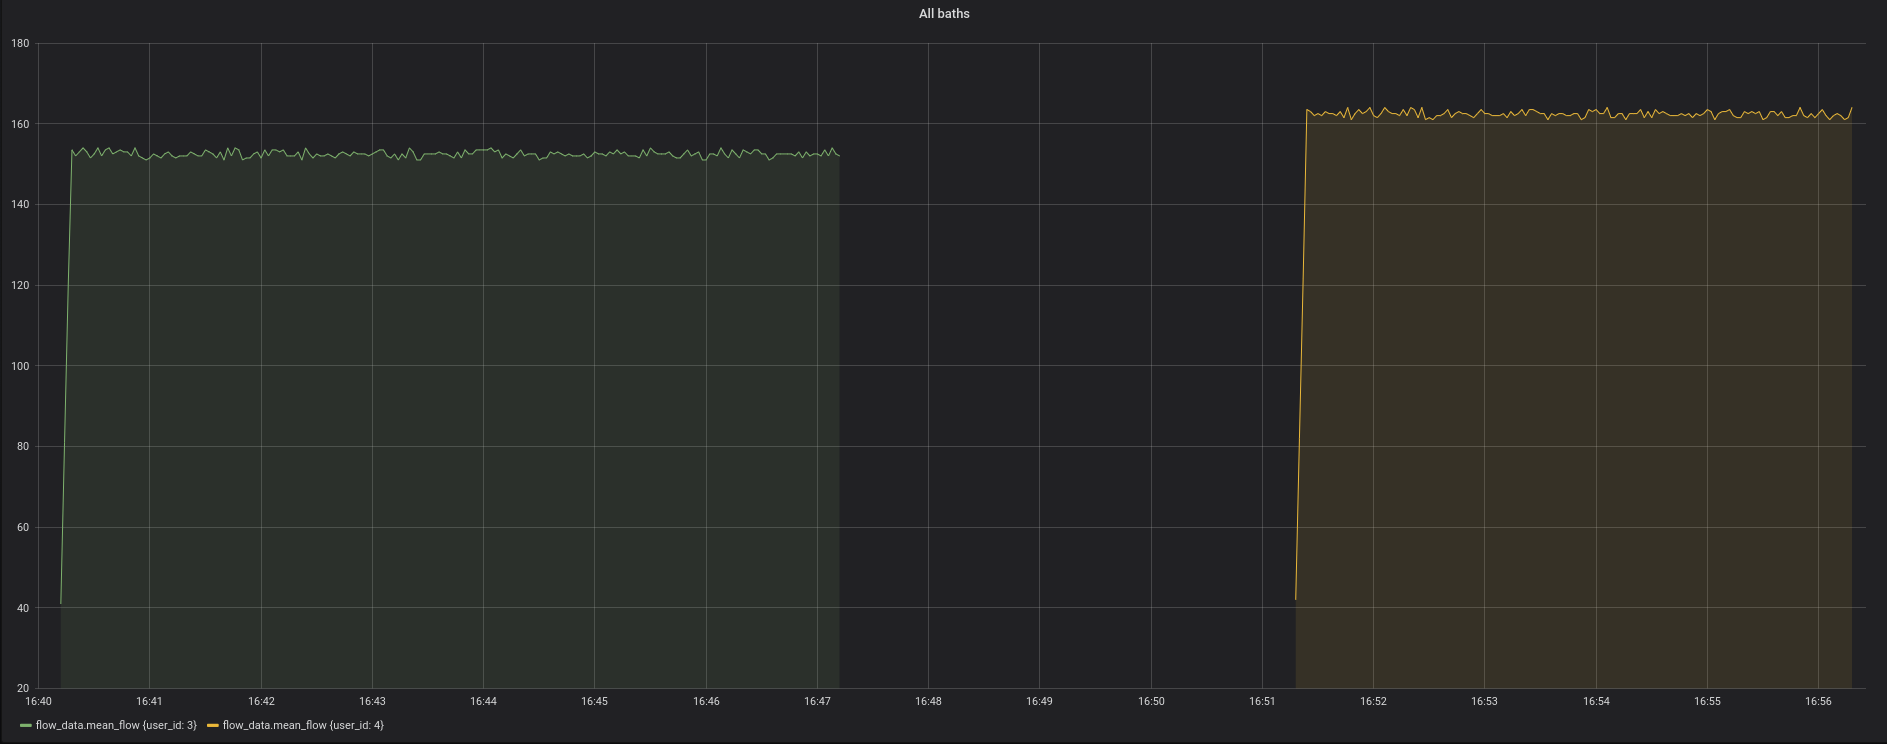
\includegraphics[width=1\linewidth]{figuras/grafanagraph.png}
	\caption{Exemplo do gráfico no Grafana para usuários diferentes.}
	\label{fig:grafana-graph}
\end{figure}

\section{Estado do atuador via HomeAssistant}

O HomeAssistant é acessado via http://localhost:8123. Ao acessar o link, observamos os estado dos sensores dos usuários cadastrado na Figura \ref{fig:homeassistant-off}, que encontram-se em estado desligado. Ao digitar corretamente a senha, o estado do sensor muda para ligado, como observado na Figura \ref{fig:homeassistant-on}.

\begin{figure}[htbp]
	\centering
	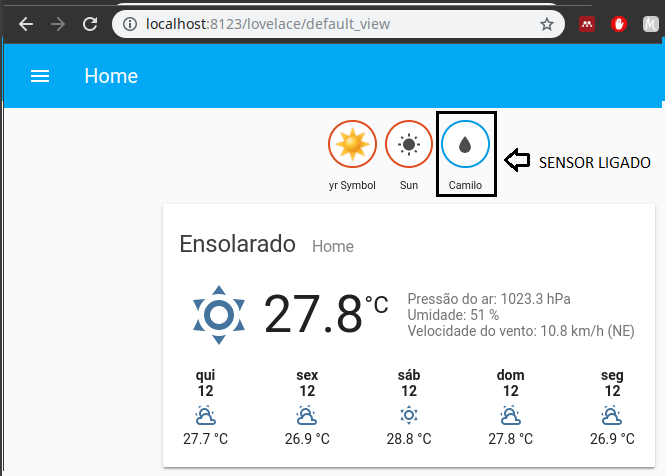
\includegraphics[width=0.6\linewidth]{figuras/homeassistanton.png}
	\caption{Exemplo do sensor no HomeAssistant quando ligado.}
	\label{fig:homeassistant-on}
\end{figure}

\begin{figure}[htbp]
	\centering
	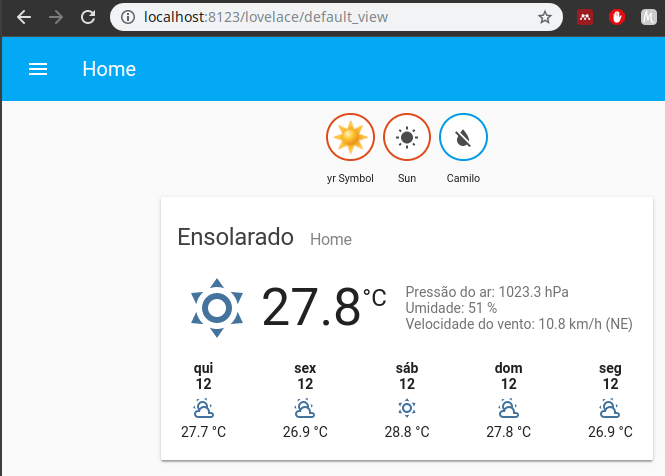
\includegraphics[width=0.6\linewidth]{figuras/homeassistantoff.png}
	\caption{Exemplo do sensor no HomeAssistant quando desligado.}
	\label{fig:homeassistant-off}
\end{figure}

Ao cadastrar um usuário, o seu sensor é inserido no HomeAssistant automaticamente (Figura \ref{fig:homeassistant-new}).

\begin{figure}[htbp]
	\centering
	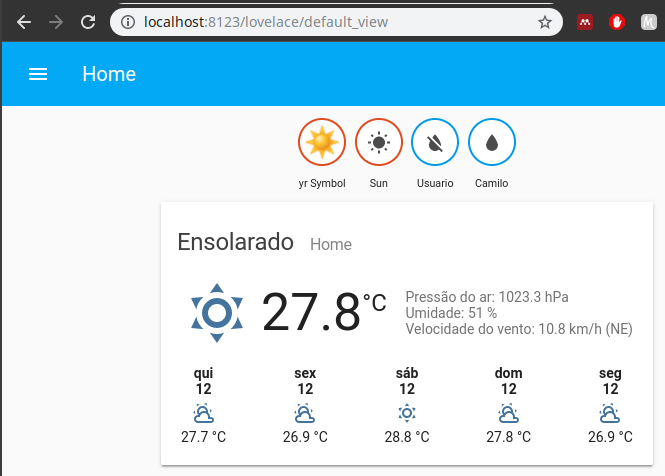
\includegraphics[width=1\linewidth]{figuras/homeassistantnewuser.png}
	\caption{Exemplo de um novo sensor quando um novo usuário é cadastrado.}
	\label{fig:homeassistant-new}
\end{figure}


